\section{Pseudosolutions and its applications. Linear regression.}
\par 
Let's repeat main possible situation for solving linear equations task, which one can be written by the next notation:
\[
    A\vec{x} = b,  
\]
where $A \in M_{m\times n}(\C), \ \vec{b} \in \C^m, \ \vec{x} \in \C^n$.
\begin{itemize}
    \item[0. ] The first case is about square matrix $A \in M_{n\times n}(\C), \ \rank A = n$. In such situation we can easily obtain unique $\overline{x}$ by inverting the matrix of initial coefficients:
    \[
        \overline{x}  = A^{-1}\vec{b}.
    \]
    \item[1. ] The next easy option is a definite system, when $A \in M_{m\times n}(\C), \rank A=n$. Then unique $\hat{x}$ can be expressed by the following ideas.
\end{itemize}

    \begin{wrapfigure}[15]{l}{0.5\columnwidth}
        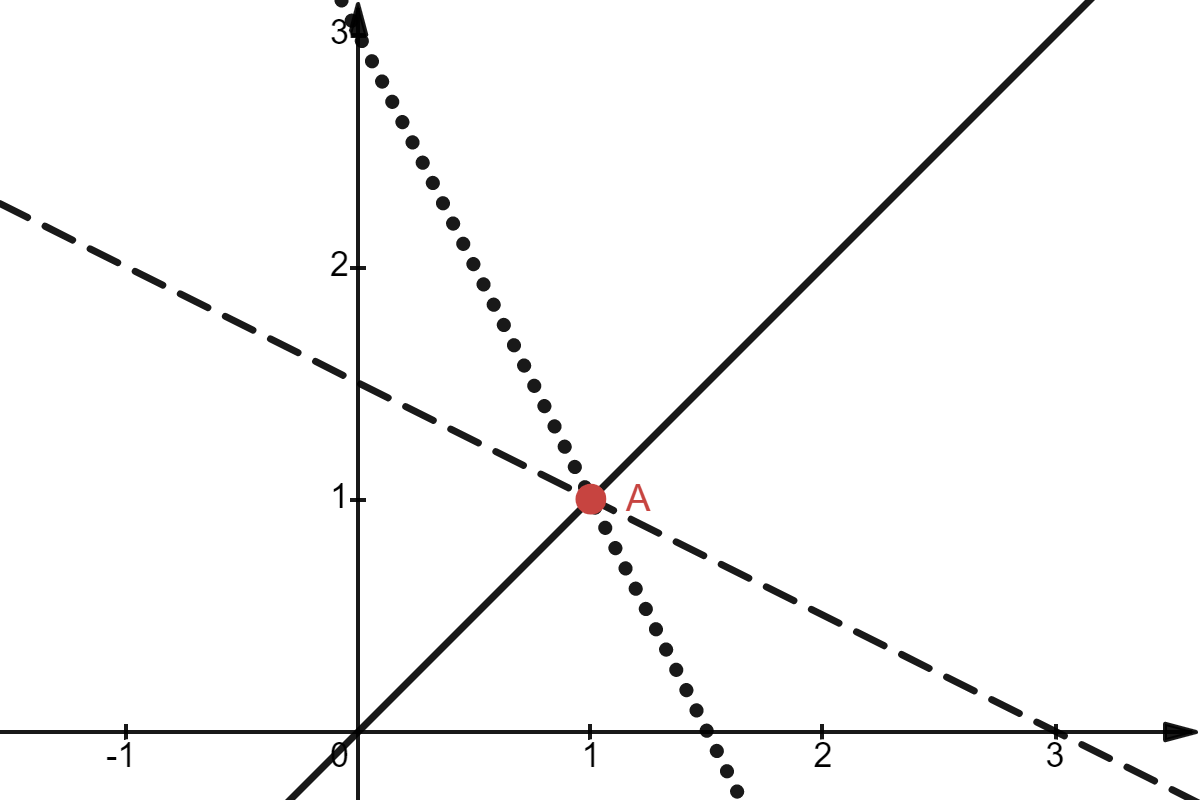
\includegraphics[height=0.333\columnwidth, width=0.5\columnwidth]{lectures/images/definite_system.png}
        \caption*{\scriptsize{Example of definite system.}}
        \label{fig:definite_system}
    \end{wrapfigure}
    Consider a system of the form:
    \[
        \left\{
            \begin{array}{l}
                2x+y = 3,\\
                x+2y = 3,\\
                x-y = 0.
            \end{array}
        \right.  
    \]
    It is obviously that system have only one correct solution in the point $A$ and it is a solution of a type: $\hat{x} = \begin{bmatrix}
        1\\ 1
    \end{bmatrix}$. However, we would like to generalize the method of obtaining a solution in such a way that it looks similar to the first (zero) case, namely:
    \[
        \hat{x} = ?\cdot \vec{b}.  
    \]

    And looking ahead we can obtain such a factor to express solution that way. But now let's get a broader generalization.
    \begin{itemize}
        \item[2. ] Also we can obtain an indefinite solution, that can provide us an infinite amount of solutions.
    \end{itemize}

    \begin{wrapfigure}[12]{r}{0.5\columnwidth}
        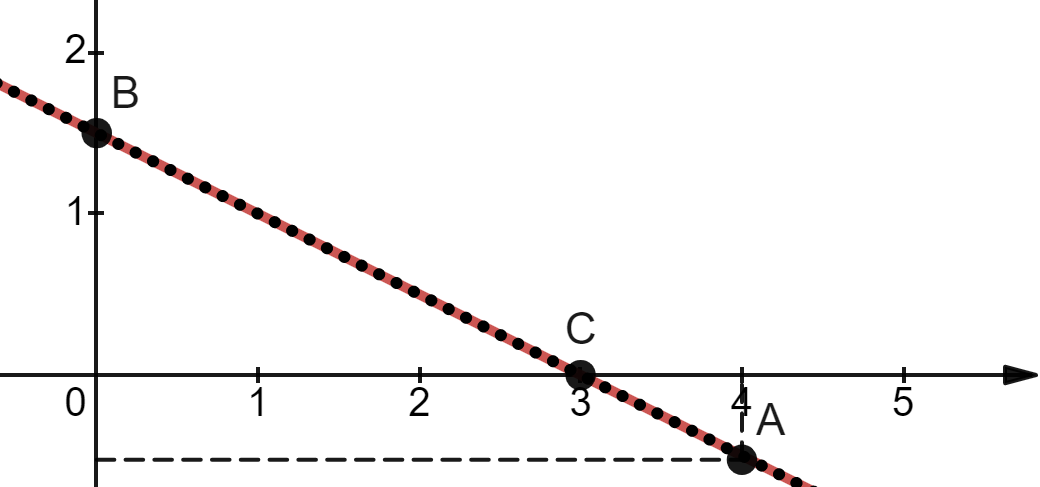
\includegraphics[height=0.235\columnwidth, width=0.5\columnwidth]{lectures/images/indefinite_system.png}
        \caption*{\scriptsize{Example of definite system.}}
        \label{fig:indefinite_system_1}
    \end{wrapfigure}
    Consider a system of two equations:
    \[
        \left\{
            \begin{array}{l}
                x+2y=3,\\
                2x+4y = 5.
            \end{array}
        \right.  
    \]

    It is not so obvious to choose a specific solution here because a whole family of solutions of the following form $\hat{x} = \begin{bmatrix}
        3-2y\\y
    \end{bmatrix}$ is suitable for us. 
    \par 
    And now we need to get some understanding about which solution is a kind of optimum. We will discuss it a little bit later, now let's consider one more possible situation.
    \begin{itemize}
        \item[3. ] 
    \end{itemize}

    \begin{wrapfigure}[18]{r}{0.4\columnwidth}
        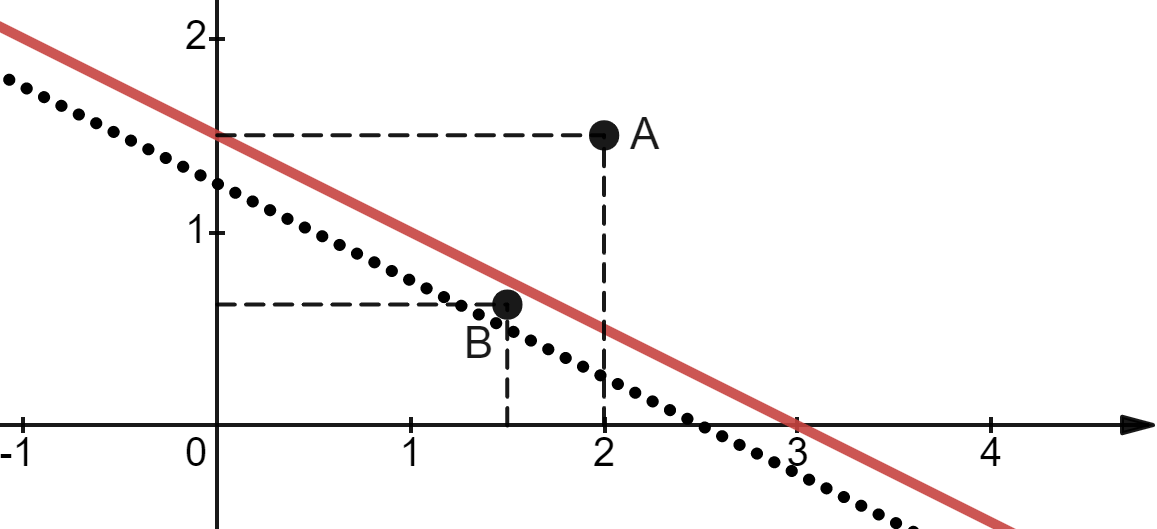
\includegraphics[height=0.45\columnwidth, width=0.36\columnwidth]{lectures/images/inconsistent_system.png}
        \caption*{\scriptsize{Example of inconsistent system.}}
        \label{fig:inconsistent_with_vectors}
    \end{wrapfigure}
    Inconsistent system is a system of a kind:
        \[
            \left\{
                \begin{array}{c}
                    2x+y=3,\\
                    2x+y=6
                \end{array}
            \right.  
        \]
    Need to remind, that we want to obtain solution in term of factors:
    \[
         \hat{x} = ? \cdot \vec{b}.
    \]
    There we have matrix and vector of initial values \[A = \begin{bmatrix}
        2 & 1\\
        2 & 1
    \end{bmatrix} \ \text{ and }\ \vec{b} = \begin{bmatrix}
        3 \\ 6
    \end{bmatrix}.\] 
    Manually we can understand that the best solution will lie somewhere between two parallel lines, perhaps even exactly in the middle. But it is still a whole family of solutions that can be the answer to the request of the product or business problem. We need a general variant to find the best solution. For this we introduce the definition:
    \par
    \begin{definition}{}{}
        Consider a system of a linear equations $A\vec{x} = \vec{b} \ \left(A \in M_{m\times n}(\C)\right)$. A vector $\vec{u} \in \C^n$ is called a pseudosolution or a least square solution, if $\forall \vec{x} \in \C^n$ the length of $A\vec{u} - \vec{b}$ is less or equal to the length of $A\vec{x} - \vec{b}$:
        \[
            \left| A\vec{u} - \vec{b} \right| \leq \left| A\vec{x} - \vec{b} \right|. 
        \]
        That is: if $f_x = \begin{bmatrix}
            f_1 \\
            \vdots\\
            f_n
        \end{bmatrix} = A\vec{x}-\vec{b}$, then $|f_x|^2 = |f_1|^2 + \ldots + |f_n|^2$ for $\vec{x}=\vec{u}$ is minimal.
    \end{definition}
    \begin{theorema}{}{}
        The vector $\vec{u} = A^+\vec{b}$ is a pseudosolution of the system of linear equations $A\vec{x} = \vec{b}$. Moreover, among all pseudosolutions, $\vec{u}$ has the minimal length.
    \end{theorema}
    \begin{proposition}{}{}
        If $\hat{x}$ is a solution, then it is a pseudosolution.
    \end{proposition}
    \begin{proof}
        $A\hat{x} - \vec{b} = 0 \Longrightarrow \left| A\hat{x} - \vec{b} \right| = 0 = \min |f_x|^2.$
    \end{proof}
    \vspace*{0.2cm}

    \Ex 
    \begin{center}
        \begin{tabular}{|c|c|}
            \hline
            Type of a system & Solution \\ \hline
            definite         &      $\vec{u} = \hat{x}$  is the solution  \\ \hline
            indefinite       &   $\vec{u} = \hat{x}$  is the solution of minimal length       \\ \hline
            inconsistent     &    $\vec{u} = \hat{x}$  is the pseudosolution  of minimal length    \\ \hline
            \end{tabular}
    \end{center}
    \begin{proof} (Of the theorem) In proof we will use
        \begin{theorema}{(Pythagoras)}{}
            Suppose $\vec{a} \perp \vec{b}$, that is $(\vec{a}, \vec{b}) = 0$. Then for $\vec{c} = \vec{a} + \vec{b}: \ |\vec{c}|^2 = |\vec{a}|^2 + |\vec{b}|^2.$ In particular $|\vec{c}| \geq |\vec{a}|$. The equality holds only for $\vec{b} = \vec{0}$.
        \end{theorema}        
        \begin{lemma}{}{}
            $\im A \perp \im B$, where $B = AA^+-I$.
        \end{lemma}

        \begin{wrapfigure}[20]{l}{0.3\columnwidth}
        \tikzset{every picture/.style={line width=1pt}} %set default line width to 0.75pt        
        \hspace*{1.5cm} \scalebox{1.25}{\begin{tikzpicture}[x=0.75pt,y=0.75pt,yscale=-1,xscale=1]
        %uncomment if require: \path (0,300); %set diagram left start at 0, and has height of 300

        %Shape: Circle [id:dp6605284406961527] 
        \draw   (100,122.75) .. controls (100,91.68) and (125.18,66.5) .. (156.25,66.5) .. controls (187.32,66.5) and (212.5,91.68) .. (212.5,122.75) .. controls (212.5,153.82) and (187.32,179) .. (156.25,179) .. controls (125.18,179) and (100,153.82) .. (100,122.75) -- cycle ;
        %Shape: Polygon [id:ds7845026568435469] 
        \draw  [pattern=_xen0kut1n,pattern size=6pt,pattern thickness=1pt,pattern radius=0pt, pattern color={rgb, 255:red, 0; green, 0; blue, 0}] (177.79,102.82) -- (204.29,125.82) -- (154.5,166.57) -- (124.5,146.57) -- cycle ;
        %Shape: Diamond [id:dp1953817249032601] 
        \draw  [pattern=_vilei2kdf,pattern size=6pt,pattern thickness=1pt,pattern radius=0pt, pattern color={rgb, 255:red, 0; green, 0; blue, 0}] (128.07,80.42) -- (162.82,98.03) -- (161.31,136.96) -- (126.57,119.35) -- cycle ;
        % Text Node
        \draw (175.5,83.37) node [anchor=north west][inner sep=0.75pt]   [align=left] {$\displaystyle \mathbb{C}^{n}$};
        % Text Node
        \draw (169.62,157.24) node [anchor=north west][inner sep=0.75pt]  [rotate=-320] [align=left] {$\displaystyle \im A$};
        % Text Node
        \draw (136,69.37) node [anchor=north west][inner sep=0.75pt]   [align=left] {$\displaystyle \im B$};
        \end{tikzpicture}}
\end{wrapfigure}

We should prove: each column $A^j$ of $A$ is orthogonal to the one $B^l$ of B.
\begin{gather*}
    \text{OR: } \forall l \ \left(B^l, A^j\right) \overset{?}{=} 0, \ \text{ or }\ B^{l^*}\cdot A^j  \overset{?}{=} 0, \\
    \text{or } \ (B^*)_l \cdot A^j \overset{?}{=} 0,\ \text{ or } \ B^*A \overset{?}{=} 0. \\
    \left(\left(AA^+\right)^* - I^*\right)A = \left(AA^+ - I\right)A = AA^+A - A = 0.
\end{gather*}
    \end{proof}